\documentclass[a4paper,11pt]{article}

\usepackage[T1]{fontenc}

\usepackage[utf8]{inputenc}

\usepackage[italian]{babel}

\usepackage{graphicx}

\usepackage{indentfirst}

\usepackage{amsmath,amssymb}

\usepackage{enumitem} 

\newcommand{\virgolette}[1]{``#1''}

\usepackage[margin=1in]{geometry} %Smaller margins

\usepackage{lmodern} %Vector PDF

\usepackage{siunitx}

\usepackage{xcolor}

\usepackage{colortbl}

\usepackage{multirow}

\usepackage{rotating}

\usepackage{booktabs}

\usepackage{longtable}

\usepackage{graphicx}
\graphicspath{ {../../Immagini/} }

\usepackage{wrapfig}

\usepackage{siunitx} % Per unit� di misura in generale e la corretta rappresentazione dei numeri.

\usepackage{gensymb} % Per il simbolo di gradi

\begin{document}
	
	\begin{equation}\label{eqn:D}
	D = D_1 + D_2 + D_3 \quad \sigma_D = \sqrt{\sigma_{D_1}^2 + \sigma_{D_2}^2 + \sigma_{D_3}^2}
	\end{equation}
	
	\begin{equation}\label{eqn:a}
	a = s_{spr} - s_{f_2} \quad \sigma_a = \sqrt{ \sigma_{s_{spr}}^2+\sigma_{s_{f_2}}^2}
	\end{equation}
	
	Da mettere da qualche parte!
	\begin{equation}\label{eqn:c}
	c = \dfrac{4 f_2 D^2 \left(\omega - \omega_0 \right)}{\left(D + a - f_2\right)\Delta\delta}
	\end{equation}
	
	\begin{equation}\label{eqn:sigmac}
		\sigma_{c_{sist}} = \sqrt{\left(\frac{\partial c}{\partial D}\right)^2\sigma_D^2+
			\left(\frac{\partial c}{\partial a}\right)^2\sigma_a^2+\left(\frac{\partial c}{\partial _2}\right)^2\sigma_{f_2}^2}
	\end{equation}
	
	\begin{equation}\label{eqn:cderivD}
	\frac{\partial c}{\partial D}=\dfrac{4Df_2(2a+D-2f_2)(\omega-\omega_0)}{(a+D-f_2)^2\Delta\delta}
	\end{equation}
	\begin{equation}\label{eqn:deriva}
	\frac{\partial c}{\partial a} = - \dfrac{4D^2f_2(\omega-\omega_0)}{\left(a+D-f_2\right)^2\Delta\delta}
	\end{equation}
	\begin{equation}\label{eqn:derivf2}
	\frac{\partial c}{\partial f_2}=\frac{4D^2(a+D)(\omega-\omega_0)}{(a+d-f_2)^2\Delta\delta}
	\end{equation}

	\subsection{Stima delle distanze}\label{sec:dist}
	\subsubsection{Verifica compatibilità} \label{subsubsec:vercomp}
	\begin{figure}
		\centering
		\caption{\emph{Clockwise} data set}
	%	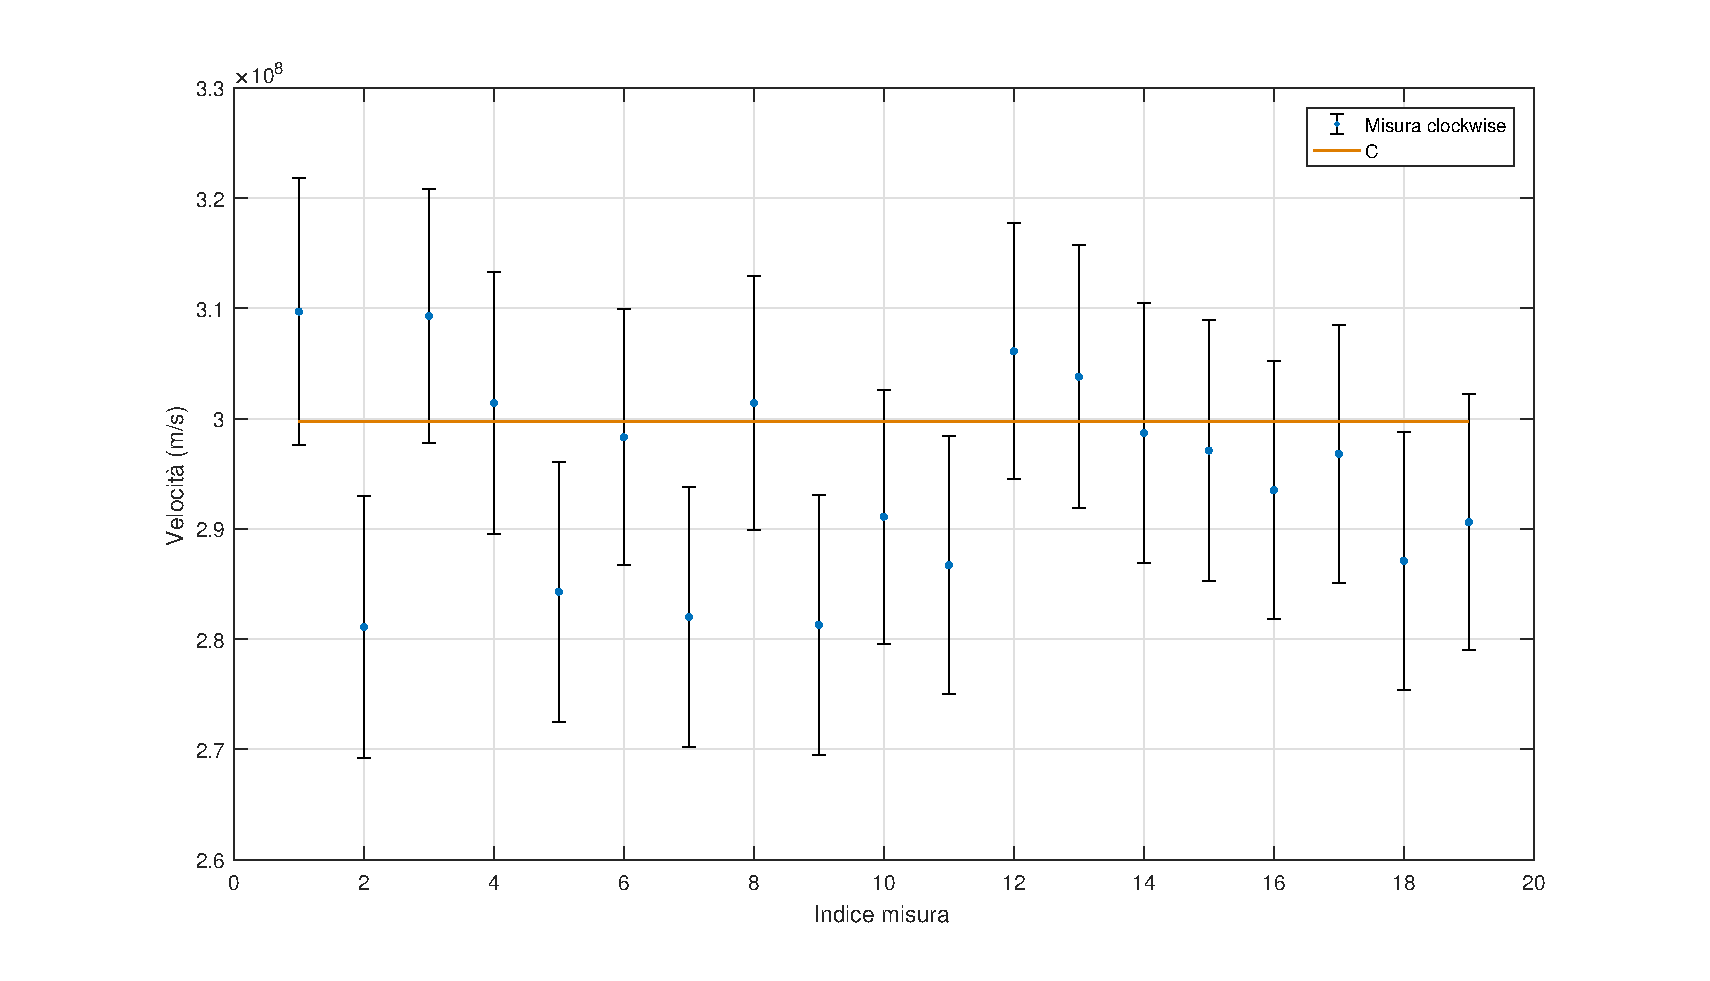
\includegraphics[width=.98\textwidth]{Clockwiseplot}
		\label{fig:clockwiseplot}
	\end{figure}
	
	
	\begin{figure}
		\centering
		\caption{\emph{Counterclockwise} data set}
	%	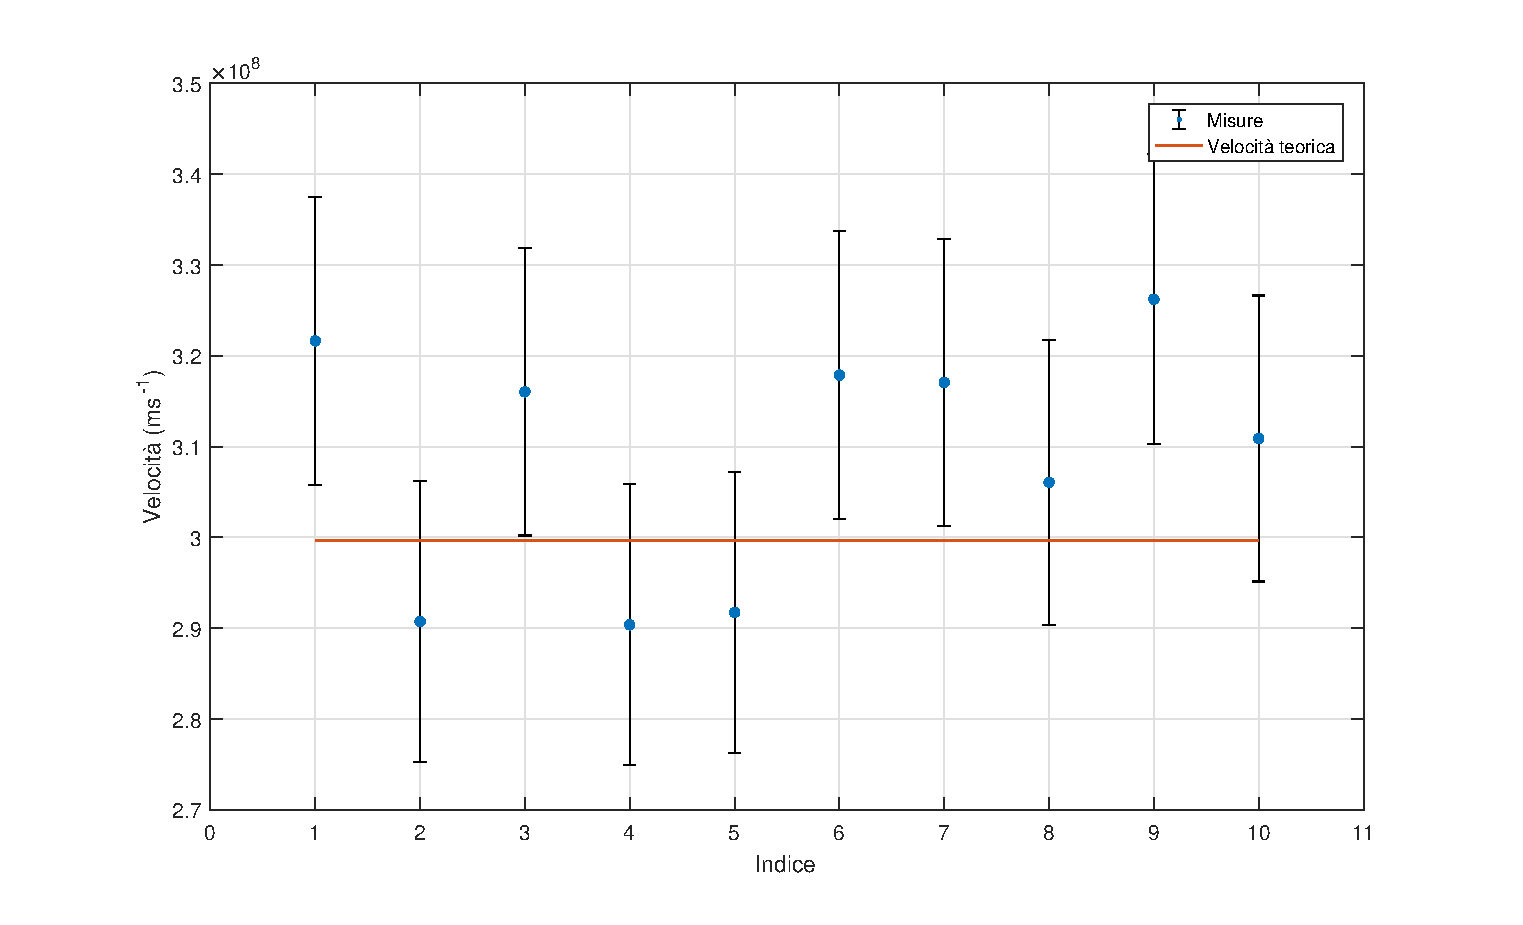
\includegraphics[width=.98\textwidth]{Counterclockwiseplot}
		\label{fig:counterclockwiseplot}
	\end{figure}
	
	\begin{figure}
		\centering
		\caption{\emph{Counterclock-clockwise} data set}
	%	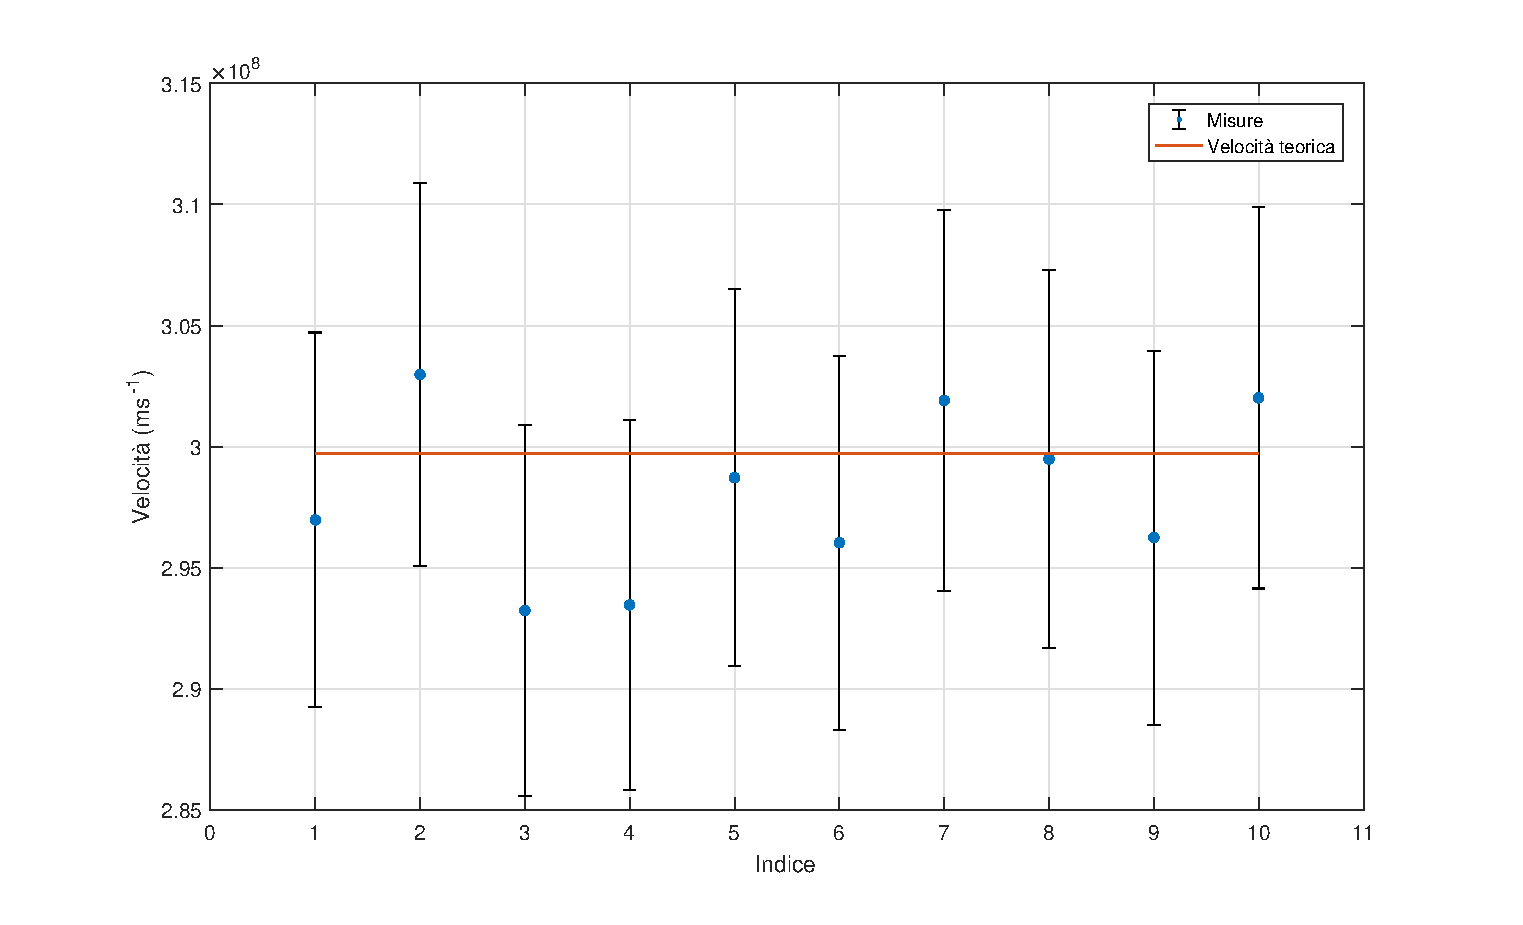
\includegraphics[width=.98\textwidth]{Clock-anticlockplot}
		\label{fig:clock-anticlockplot}
	\end{figure}
	
	Per una corretta visualizzazione dei numeri, con le unità di misura e gli ordini di grandezza usare il pacchetto siunitx con i comandi:\\
	
		\SI{5}{\centi\meter}
	\\
		\SI{633e-9}{\meter}
	\\
		\num{6.022e23}
	\\
	Inoltre usiamo la convenzione internazionale per cui i decimali si separano con un punto per piacere.
	

	
\end{document}
